1章の本文です.

参考文献の例\cite{Koren1991,山下2018,Lavalle1998,坂原2007}です.
図\ref{fig:outline}は図の例です.
表\ref{tab:accuracy}は表の例です.
式(\ref{eq:lsm})は数式の例です.


%----------------------------------------------
\begin{figure}[tb]
    \begin{center}
        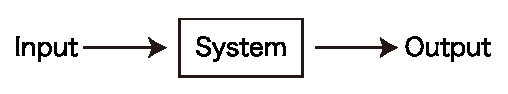
\includegraphics[width=80mm]{figure/eps/outline.eps}
        \caption{提案手法の流れ.}
        \label{fig:outline}
    \end{center}
\end{figure}
%----------------------------------------------



%----------------------------------------------
\begin{table}[tb]
  \begin{center}
    \caption{提案手法と従来法の認識精度の比較.}
    \label{tab:accuracy}
    \begin{tabular}{c|c|c} \hline
      シーケンス番号& 提案手法[\%] & 従来法[\%] \\ \hline 
      1 & 62.3 & 60.2  \\
      2 & 83.2 & 85.0 \\
      3 & 78.8 & 42.7 \\ \hline
    \end{tabular}
  \end{center}
\end{table}
%----------------------------------------------

%----------------------------------------------
\begin{equation}
\label{eq:lsm}
    A = \frac{Cov(X,Y)}{\sigma_x^2} \\
    B = \mu_Y - A\mu_X
\end{equation}
%----------------------------------------------

